We may rewrite the equation \ref{eq: mb_distribution} as a function of the mean velocity $\bar{v}$ into a simpler form .

\begin{equation}
	f(v) = \frac{32}{\pi^2} \frac{v^2}{\bar{v}^3} e^{-4v^2/\pi \bar{v}^2} \label{eq: mb_simplified}
\end{equation}

To get the velocity distribution in the beam, we can calculate the distribution of particles incident on an aperture in the cell.

\begin{align*}
	f_{beam}(v) & = \frac{v}{\bar{v}}f(v)  \\
	& = \frac{32}{\pi^2} \frac{v^3}{\bar{v}^4} e^{-4v^2/\pi \bar{v}^2}
\end{align*}

For low Reynold's numbers (Re<1) the flow at the aperture is purely molecular, which means that there are few to no collisions. This allows us to continue to use the Maxwell-Boltzmann distribution to describe the forward velocity \cite{Hutzler2011c}.

\begin{equation}
	\bar{v}_\parallel = \int_0^\infty v f(v) dv \approx 1.2 \bar{v}
\end{equation}

The spread of the forward velocity of an effusive beam is the full width half max (FWHM) of the Maxwell-Boltzmann distribution: $\Delta\bar{v} \approx 1.5 \bar{v}$. As the Reynolds number increases, one can reach the supersonic regime (Re>100) where the forward velocity reaches $1.4\bar{v}$ and the distribution drastically narrows.\cite{Hutzler2011c,Pauly}

But as the flow regime nears the supersonic regime, forward collisions around the aperture cause boosting of the average velocity as well as a decrease in the velocity spread. Changing the flow regime may also change the ratio of species in the beam as well.

A helium buffer gas held at 4K will have a slower forward velocity than that of a neon gas held at 17K. Despite this, it is preferable to use neon as a buffer gas due to its ideal cryopumping properties. Helium requires large amounts of activated charcoal, also held at low temperatures, to effectively cryopump. These volumes of charcoal can then become saturated and require purging, limiting one's operating time (few hours). Neon on the other hand, only requires a metal surface lower than 17K to create neon ice. The neon ice surface will then act as a cryopump for more neon gas as well, allowing for many hours of continuous operation with no appreciable build up of background gas. Our experiment uses neon as a buffer gas for its technical simplicity, the lower achievable temperature with the helium does not yield dramatic gains in the final reaction temperature.

To better understand the reaction temperatures we will be able to reach, we need a characterization of the beam's velocity, more specifically, the velocity of the target species entrained within the buffer gas. By ablating ytterbium into the neon buffer gas, we find that the ytterbium is entrained within the neon and sympathetically cooled to the cell's temperature. As long as the target species number density is a trace amount in comparison to the bulk buffer gas number density (0.1\%), the flow characteristics are dominated by the buffer gas species \cite{Hutzler2012}. The forward velocity of the beam is not only parameterized by the temperature of the buffer gas species, it is also dependent on the flow regime. As we increase the flow of neon into the cell, figure \ref{fig: rga} shows a linear increase in the \ce{H2O} signal from a downstream RGA. This coincides with the beam operating within the intermediate flow regime, where there are few collisions at the cell aperture, resulting in a slight forward boosting and increased extraction efficiency of the target species. At higher flow regimes, entering the supersonic regime, we would see a "freeze out" where the forward velocity reaches $1.4\bar{v}$ and we would not see appreciable gains in species extraction \cite{Hutzler2012}. We chose to operate at a nominal neon flow rate of 30SCCM based upon the reaction rate of the ions downstream.

\begin{figure}[H]
	\centering
	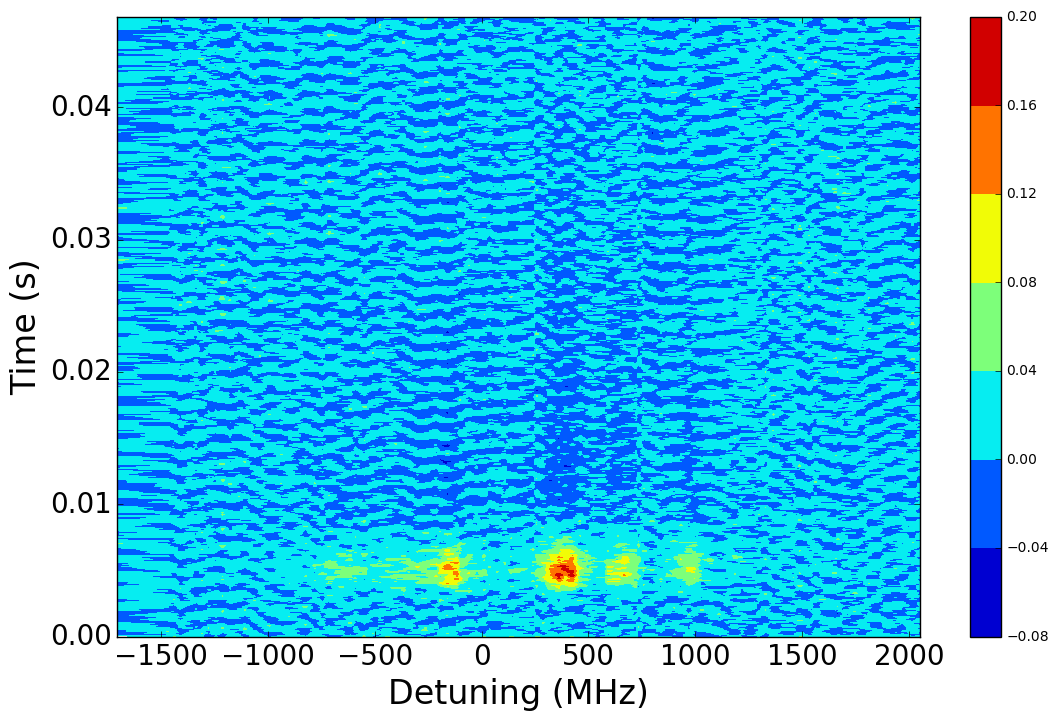
\includegraphics[width=1\textwidth]{images/CBGB_Yb_spectrum_scan.png}
	\caption{}
	\label{fig: yb_spectrum_scan}
\end{figure}
\todo{find appropriate plot}

\begin{figure}[H]
	\centering
	\includegraphics[width=1\textwidth]{images/CBGB_Yb_spectrum_long.png}
	\caption{}
	\label{fig: yb_spectrum}
\end{figure}